\newcommand{\proofsketch}{\smallskip\noindent{\bf Proof sketch. }}
\algrenewcommand\algorithmicfunction{\textbf{Machine}}
\newcommand{\bits}{\set{0,1}}
\newcommand{\Ex}{\mathbb{E}}

\renewcommand{\O}{\ensuremath{\mathcal{O}}}
\newcommand{\To}{\rightarrow}
\newcommand{\e}{\epsilon}
% \newcommand{\R}{\mathbb{R}}
\newcommand{\N}{\mathbb{N}}
\newcommand{\Z}{\mathbb{Z}}
\newcommand{\logAnd}{\wedge}

\newcommand{\indis}{\mathrel{\overset{\makebox[0pt]{\mbox{\normalfont\tiny c}}}{\approx}}}
\newcommand{\allindis}{\mathrel{\overset{\makebox[0pt]{\mbox{\normalfont\tiny p/s/c}}}{\approx}}}

\newcommand{\cclass}[1]{\mathsf{#1}}
\renewcommand{\P}{\cclass{P}}
\newcommand{\NP}{\cclass{NP}}
\newcommand{\Time}{\cclass{Time}}
\newcommand{\BPP}{\cclass{BPP}}
\newcommand{\Size}{\cclass{Size}}
\newcommand{\Ppoly}{\cclass{P_{/poly}}}
\newcommand{\CSAT}{\ensuremath{\mathsf{CSAT}}}
\newcommand{\SAT}{\ensuremath{\mathsf{3SAT}}}
\newcommand{\IS}{\mathsf{INDSET}}



\newcommand{\inp}{\mathsf{in}}
\newcommand{\outp}{\mathsf{out}}

\newcommand{\Param}{\kappa}
\newcommand{\Adv}{\mathsf{Adv}}
\newcommand{\Supp}{\mathsf{Supp}}


\newcommand{\PRG}{\mathsf{G}}
\renewcommand{\Enc}{\mathsf{Enc}}
\renewcommand{\Dec}{\mathsf{Dec}}
\renewcommand{\sk}{\mathsf{sk}}
\newcommand{\sfC}{\mathsf{C}}
\newcommand{\sfR}{\mathsf{R}}

\newcommand{\eqdef}{\stackrel{\text{\tiny def}}{=}}

\newcommand{\cF}{\mathcal{F}}

\newcommand{\angles}[1]{\langle #1 \rangle}
\newcommand{\iprod}[1]{\angles{#1}}

\newcommand{\Com}{\mathsf{Com}}


% Real vs. Ideal
\newcommand{\RealAdv}{\mathcal{A}}
\newcommand{\IdealAdv}{\mathcal{S}}
\newcommand{\RealVar}{\mathsf{Real}}
\newcommand{\IdealVar}{\mathsf{Ideal}}

\newcommand{\RealView}[2]{\mathsf{Real}^{#1}_{#2}}
\newcommand{\IdealView}[2]{\mathsf{Ideal}^{#1}_{#2}}

% Participating parties
\newcommand{\PartyA}{P_1}
\newcommand{\PartyB}{P_2}
\newcommand{\InputA}{x_1}
\newcommand{\InputB}{x_2}


% Garbling Schemes
\newcommand{\Garble}{\mathsf{Garble}}
\newcommand{\Cir}{C}
\newcommand{\GCir}{\widetilde{C}}
\newcommand{\Lab}{\mathsf{lab}}

% Proof
\newcommand{\Sim}{\mathsf{Sim}}

% GMW

% Misc
\newcommand{\out}{\mathsf{out}}
\newcommand{\Assign}{:=}

\chapter{Secure Computation}

\section{Introduction}
Secure multiparty computation (or MPC) considers the problem of enabling mutually distrusting parties
to compute a joint public function on their private inputs without revealing
any extra information about these inputs beyond what is leaked by the output
of the computation.
For instance, there could be three parties $P_1, P_2, P_3$ with private inputs $x_1, x_2, x_3$ respectively, and they want to compute a public function $f$ without revealing anything beyond $f(x_1, x_2, x_3)$.
Note that this notion generalizes zero knowledge proofs, where the prover's input is the statement-witness pair $(x, w)$, the verifier's input is the statement $x$, and the public function $f$ is the verification algorithm for the corresponding relation which outputs $1$ if $w$ is a valid witness w.r.t. $x$.

This setting is well motivated, and captures many different applications.
Now, we look at some applications of MPC which will help build intuition and also highlight the challenge in defining security for MPC.
% Considering some of these applications will provide intuition about how security should be defined for secure computation:
\begin{description}
  \item[Voting:] Electronic voting can be thought of as a multi-party computation
	  between $n$ players: the voters. Their input is their choice $b \in \{0,1\}$
    (we restrict ourselves to the binary choice setting without loss of generality), and the function
    they wish to compute is the majority function.
    % Now consider what happens when only one user votes: their input is trivially revealed as the output of the computation. What does privacy of inputs mean in this scenario?

  \item[Yao's Millionaires' Problem:] Two millionaires want to know who is richer
    without revealing their actual wealth. The function they want to compute is
    $f(x_1, x_2) = x_1 > x_2$.
    % Let's say $x_2 = 1$M $+ 1$ and $f(x_1, x_2) = 0$. Then 
  
  \item[Private Contact Discovery:] Signal employs MPC to identify contacts from your phone who are also on Signal, all without exposing your contact list to Signal.
  Here the function $f$ is an intersection function over the user's contact list and Signal's member list. This specific application of MPC is commonly known as private set intersection (PSI) and has been the subject of extensive research.

  \item[Password Breaches:] Suppose your browser needs to verify whether your password has been compromised, but without disclosing it to a service that maintains a database of leaked passwords. This is also an instance of PSI.

  \item[Cryptographic Wallets:] Cryptographic wallets typically split their keys into multiple shards that are then given to multiple parties (e.g., the user's device and the wallet provider) so that compromising any one party does not reveal the keys. In principle, whenever these keys are needed, the client can get the shards from each party and perform the operation. However, the client becomes the single point of compromise for that period and that defeats the point of sharding. MPC enables the parties holding the shards to perform any operations on the keys without reconstructing it on a single device.

  \item[Searchable Encryption:] Searchable encryption schemes allow clients
    to store their data with a server, and subsequently grant servers tokens
    to conduct specific searches.
    % However, most schemes do not consider access pattern leakage. This leakage tells the server potentially valuable information about the underlying plaintext. How do we model all the different kinds information that is leaked?
\end{description}

Note that in all these applications, the output revealed to the parties itself can reveal a lot of information about the private inputs of the parties.
For instance, in the voting example, if only one user votes, their input is trivially revealed.
Or, in the case of the millionaires, if $x_1 = 10^6 + 1$ and $f(x_1, x_2) = 1$, then the first millionaire knows that $x_2 = 10^6$.
Similarly, most searchable encryption schemes do not consider access pattern leakage. This leakage tells the server potentially valuable information about the underlying plaintext.
How do we model all the different kinds information that is leaked?

From these examples we see that defining security of MPC is tricky because it is imperfect in that some leakage in inherent in the computation.
What we want to capture is that no party should learn anything about the private inputs of other parties beyond what is revealed by the output of the computation.
% We want to ensure that no party can learn anything more from the secure computation protocol than it can from just its input and the result of the computation.
To formalize this notion, we adopt the \textbf{real/ideal world paradigm}.



\section{Real/Ideal World Paradigm}
Suppose there are $n$ parties and each party $P_i$ has a private input $x_i$.
They want to compute a public function (represented by circuit $C$) on their inputs.
The goal is to do this securely: even if some parties are corrupted, no party $P_i$ should learn anything beyond $y_i$ where $(y_1, \ldots, y_n) = C(x_1, \ldots, x_n)$.

\paragraph{Real World.} In the real world, the $n$ parties interact with each other and participate in a protocol $\Pi$
to compute $C$.
This protocol can involve multiple rounds of interaction.
The real world adversary $\RealAdv$ can corrupt a subset of the parties.
The interaction is summarized in Figure~\ref{fig:real-world}.

\begin{marginfigure}
  \centering
  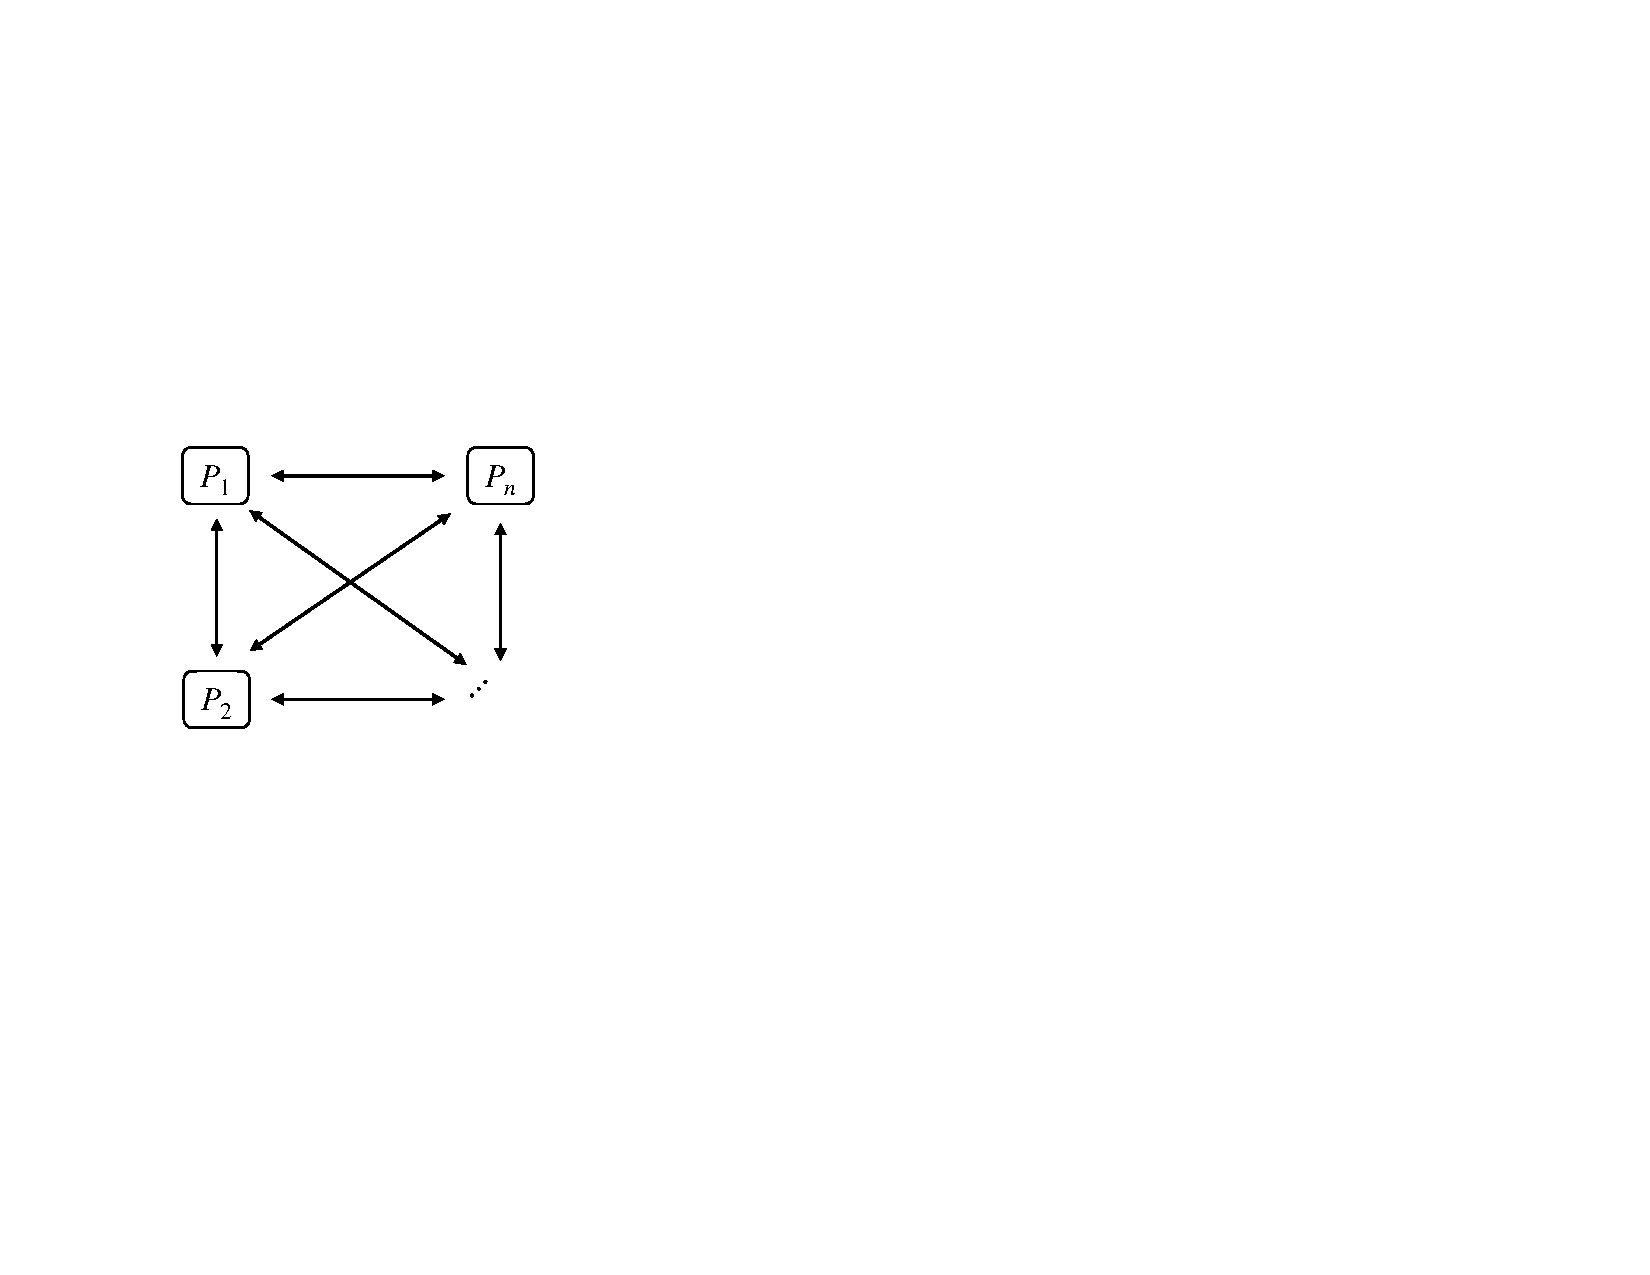
\includegraphics[width=\textwidth]{figures/real-world.pdf}
  \caption{Real world interaction.} \label{fig:real-world} 
\end{marginfigure}

\paragraph{Ideal World.} In the ideal world, an angel or trusted third party $\cF_{C}$ (parameterized by $C$) helps in the computation of $C$.
The computation in this world is secure by design:
each party $P_i$ sends its input $x_i$ to $\cF_C$ and receives the output $y_i$ of the computation $(y_1, \ldots, y_n) = C(x_1, \dotsc, x_n)$.
In this world, an ideal world adversary $\IdealAdv$ controls the parties corrupted by $\RealAdv$ in the real world, and as such, is responsible for sending their inputs to $\cF_C$.
The interaction is summarized in Figure~\ref{fig:ideal-world}.
% $\IdealAdv$ has access to the inputs of the corrupted parties and can arbitrarily choose the inputs sent to $\cF_C$.
\begin{marginfigure}
  \centering
  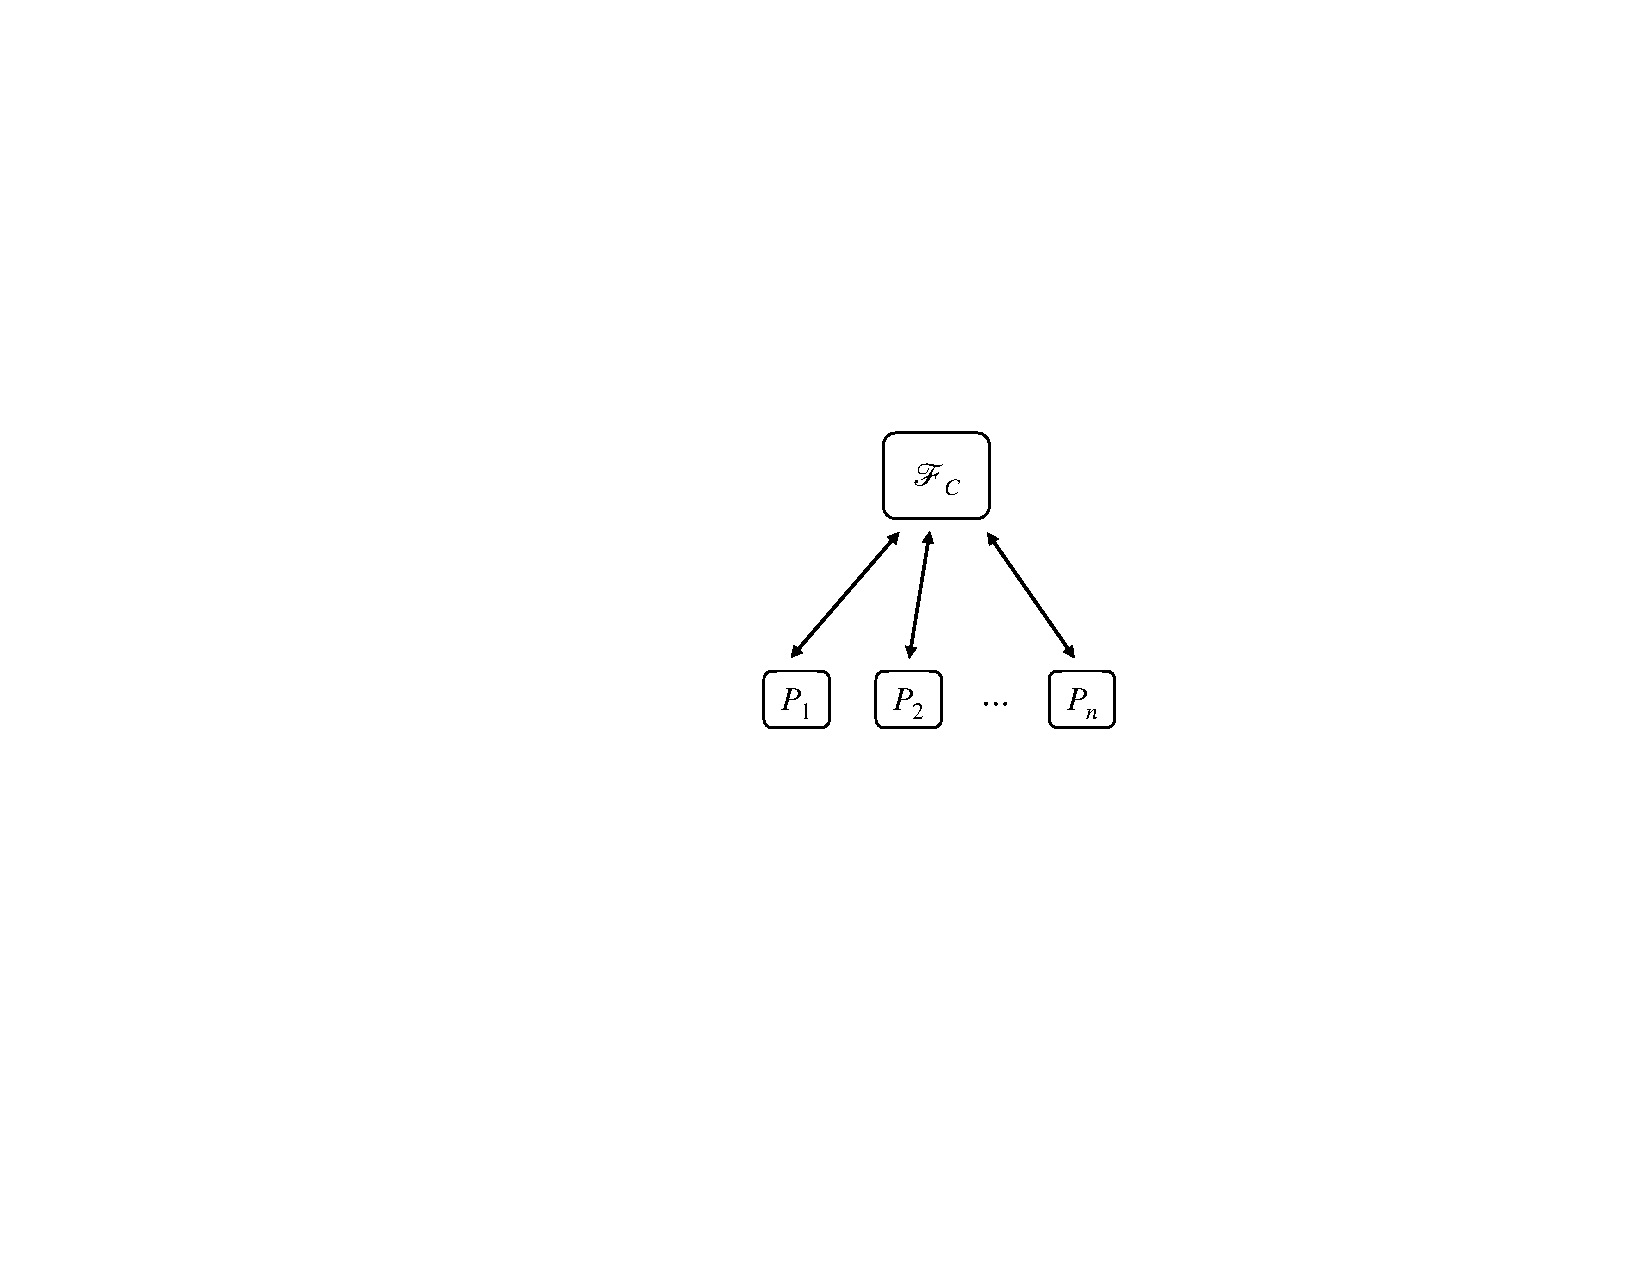
\includegraphics[width=\textwidth]{figures/ideal-world.pdf}
  \caption{Ideal world interaction.} \label{fig:ideal-world} 
\end{marginfigure}

% To model malicious adversaries, we need to modify the ideal world model as follows. 
% Some parties are honest, and each honest party $P_i$ simply sends $x_i$ to the angel. The other parties are corrupted and are under control of the adversary $\IdealAdv$. The adversary chooses an input $x_i'$ for each corrupted party $P_i$ (where possibly $x_i' \neq x_i$) and that party then sends $x_i'$ to the angel. The angel computes a function $f$ of the values she receives (for example, if only party 1 is honest, then the angel computes $f(x_1, x_2', x_3', \dotsc, x_n')$) in order to obtain a tuple $(y_1, \dotsc, y_n)$. 
% She then sends $y_i$ of corrupted parties to the adversary, who gets to decide whether or not honest parties will receive their response from the angel. The angel obliges. Each honest party $P_i$ then outputs $y_i$ if they receive $y_i$ from the angel and $\perp$ otherwise, and corrupted parties output whatever the adversary tells them to. 

\paragraph{Notation.}
Let $\lambda$ denote the security parameter. Let $\RealView{\RealAdv}{\Pi}(1^\lambda, x_1, \ldots, x_n, z)$ denote the joint distribution of the honest party outputs as well as the view of the corrupted parties (randomness, inputs, outputs, all messages seen during the protocol) in the real world, where $z$ is an auxiliary inputs available to $\RealAdv$.
Let $\IdealView{\IdealAdv}{\cF_C}(1^\lambda, x_1, \ldots, x_n, z)$ denote the joint distribution of the honest party outputs in the ideal world and the protocol transcript (or view) output by ideal adversary $\IdealAdv$ given inputs and outputs of corrupted parties.

\paragraph{Security Definition.} 
A protocol $\Pi$ securely realizes $C$ if there exists a PPT ideal adversary $\IdealAdv^{\RealAdv(\cdot)}$ (with oracle access to the real world adversary) such that $\forall$ non-uniform PPT adversaries $\RealAdv$ in the real world, $\forall$ private inputs $x_1, \ldots, x_n$, and $\forall$ auxiliary inputs $z \in \bit^{\ast}$, we have:
\[ \RealView{\RealAdv}{\Pi}(1^\lambda, x_1, \ldots, x_n, z) \approx_{c} \IdealView{\IdealAdv}{\cF_C}(1^\lambda, x_1, \ldots, x_n, z) \]

% there exists an PPT adversary $\IdealAdv$ in the ideal world such that for all tuples of bit strings $(x_1, \dotsc, x_n)$, we have
% \[ \mathrm{Real}_{\Pi, \RealAdv}(x_1, \dotsc x_n) \stackrel{c}{\simeq} \mathrm{Ideal}_{F,\IdealAdv}(x_1, \dotsc, x_n) \]
% where the left-hand side denotes the output distribution induced by $\Pi$ running with $\RealAdv$, and the right-hand side denotes the output distribution induced by running the ideal protocol $F$ with $\IdealAdv$. 
% The ideal protocol is either the original one described for semi-honest adversaries, or the modified one described for malicious adversaries. 





%We require that the views of the parties
%in each of the scenarios be identical, i.e.\ that a real-world execution of the
%protocol $\Pi$ should not leak any information not leaked by the ideal-world
%execution. Hence, the parties can only learn what they can infer from their
%inputs and the output $f(\InputA, \InputB)$. More formally, assuming $\RealAdv$
%corrupts one party (say $\PartyA$, wlog), we define random variables
%$\RealVar_{\Pi, \RealAdv}(\InputA, \InputB) = \RealAdv(\InputA, r_1, \text{messages
%sent in } \Pi)$ and $\IdealVar_{F, \IdealAdv}(\InputA, \InputB) = \IdealAdv(\InputA,
%f(\InputA,\InputB))$.  These random variables represent the views of the
%adversary in each of the two settings. Our definition of security thus requires
%that
%
%\begin{equation*}
%\RealVar_{\Pi, \RealAdv}(\InputA, \InputB) \indis \IdealVar_{F, \IdealAdv}(x_1, x_2).
%\end{equation*}

\paragraph{Setting.} So far, we have brushed over some important details of the setting.
Below we state these details explicitly:
\begin{enumerate}
  \item \textbf{Assumption:} The protocol could rely on cryptographic assumptions and be secure against computationally bounded adversaries, or it could be statistically secure and protect against unbounded adversaries.
  \item \textbf{Setup:} The parties in the protocol could have access to a common reference string (CRS) that is generated by the trusted party in the ideal world.
  \item \textbf{Communication Channel:} 
  The setting could assume private peer-to-peer (P2P) channels among the parties, a broadcast channel, a combination of both, or insecure channels which don't have privacy or integrity. In the statistical setting, we assume secure P2P channels because they require computational assumptions to set up.
  \item \textbf{Corruption Type:} We consider primarily two types of adversaries:
    \begin{itemize}
      \item \emph{Semi-honest adversaries:} Corrupted parties follow the protocol
        execution $\Pi$ honestly, but attempt to learn as much information as they
        can from the protocol transcript.
      \item \emph{Malicious adversaries:} Corrupted parties can deviate arbitrarily
        from the protocol $\Pi$.
    \end{itemize}
  % We assume that the communication channel between the involved parties is completely insecure, i.e., it does not preserve the privacy of the messages. However, we assume that it is reliable, which means that the adversary can drop messages, but if a message is delivered, then the receiver knows the origin.
  \item \textbf{Corruption Model:} We have different models of how and when the
    adversary can corrupt parties involved in the protocol:
    \begin{itemize}
      \item \emph{Static:} The adversary chooses which parties to corrupt before the protocol execution starts, and during the protocol, the malicious parties remain fixed.
      \item \emph{Adaptive:} The adversary can corrupt parties dynamically during the protocol execution and the state of that honest party corrupted is given to the adversary. 
      % \item \emph{Mobile:} Parties corrupted by the adversary can be ``uncorrupted'' at any time during the protocol execution at the adversary's discretion.
    \end{itemize}
  \item \textbf{Fairness:}
  The protocol we consider could be ``fair'', i.e., if one party gets their output, then all parties get their output, or they could be unfair where a corrupted party can abort the computation after learning the output before the honest parties can learn it.
  It is important to model this weakness of the protocol in the ideal functionality $\cF_C$.
  This is done by having the ideal functionality ask the ideal adversary if the honest parties should receive an output. If adversary disapproves, the ideal functionality sends the special abort output $\bot$ to the honest parties.
  % The protocols we consider are not ``fair'', i.e., the adversary can cause corrupted parties to abort arbitrarily. This can mean that one party does not get its share of the output of the computation.

  \item \textbf{Corruption Bound:} 
  The setting places some upper bound $t$ on the total parties $n$ that can be corrupted by the adversary (there is nothing to protect when all parties are corrupted). 
  Some well-known corruption settings are $t<n$, $t<n/2$, $t<n/3$, and $t \leq \log n$.
  % In some scenarios, we place upper bounds on the number of parties that the adversary can corrupt.

  \item \textbf{Standalone vs Concurrent Execution:}
  In some settings, protocols can be executed in isolation; only one instance of a particular protocol is ever executed at any given time. In other settings, many different protocols can be executed concurrently. This can compromise security.
\end{enumerate}

\section{A Simple and Efficient MPC Protocol}
This protocol is highly efficient and considers a very simple setting: $n=3$ parties, corruption bound $t=1$, unbounded and semi-honest adversary, statistical security, unfairness, and secure P2P channels.

\noindent\textbf{(2,3)-secret sharing scheme:}
A $(n,t)$-sharing splits a secret such that any $t$ shares are enough to reconstruct the secret, and any set of less than $t$ shares do not reveal anything about the secret.
Let $k \in \mathbb{Z}_p$ be a secret. A $(3,3)$-sharing is easy to construct: sample $k_1, k_2$ uniformly at random from $\mathbb{Z}_p$ and set $k_3 = k - k_1 - k_2 \mod p$.
Given $(3,3)$-shares, we can construct a $(2,3)$-sharing by considering a replicated secret sharing scheme: each party $P_i$ gets shares $k_i, k_{i+1 \mod 3}$. It is easy to see that the shares held by any two parties are sufficient to reconstruct the secret.

\noindent\textbf{Protocol:}
The protocol proceeds in the following phases:
\begin{description}
  \item[Input Sharing Phase:] 
  Each party $P_i$ shares their input $x_i$ using the $(2,3)$-sharing scheme, and sends the corresponding shares to the other parties.
  For instance, $P_1$ shares $x_1$ as $(x_{1,1}, x_{1,2}, x_{1,3})$, keeps $(x_{1,1}, x_{1,2})$, and sends $(x_{1,2}, x_{1,3})$ to $P_2$ and $(x_{1,3}, x_{1,1})$ to $P_3$.
  \item[Computation Phase:] 
  The computation phase maintains the invariant that given $(2,3)$-shares of the input to a gate (addition or multiplication), the computation produces $(2,3)$-shares of the output of the gate. That way, the parties can keep compute the gates all the way to the output of the circuit $C$.

  \textbf{Addition Gate}:
  Addition gates are simple: given $(2,3)$-shares of $\alpha$ and $\beta$, the parties can compute $(2,3)$-shares of $\alpha + \beta$ by simply summing up their shares locally.
  For instance, party $P_1$ can compute its shares of $\alpha+\beta$ by computing $(\alpha_1 + \beta_1, \alpha_2 + \beta_2)$. 

  \textbf{Multiplication Gate}:
  Multiplication gates are more involved. The product $\gamma = \alpha \cdot \beta$ can be represented in the form of shares as follows: $\gamma = \alpha \cdot \beta = (\alpha_1 + \alpha_2 + \alpha_3) \cdot (\beta_1 + \beta_2 + \beta_3)$.
  There are nine terms in this product, and note that all parties together can compute every term given their shares of $\alpha$ and $\beta$. 
  Thus, assuming each party computes the sum of three mutually exclusive terms (let's call it $\gamma_i$ for party $P_i$), they can locally compute $(3,3)$-shares of $\gamma$.
  To go from $(3,3)$-shares to $(2,3)$-shares, each party $P_i$ can send $\gamma_i$ to party $P_{i-1 \mod 3}$.

  We are not done yet. These shares represent partial sums and can reveal information about the secret. To prevent this, each party needs to additionally mask $\gamma_i$ before sending it.
  In particular, $P_i$ does the following: (i) mask $\gamma_i$ by adding a random value $r_i$ to it before sending it to $P_{i-1 \mod 3}$, (ii) subtract $r_i$ from $\gamma_{i+1 \mod 3}$ received from $P_{i+1 \mod 3}$, and (iii) additionally send $r_i$ to $P_{i+1 \mod 3}$, who also subtracts $r_i$ from $\gamma_{i+1 \mod 3}$.

  \item[Output Reconstruction Phase:] 
  Each party simply publishes its shares of the output of the circuit $C$.
\end{description}

\begin{theorem}
  The protocol described above securely realizes the circuit $C$ in the presence of a static semi-honest adversary that corrupts at most one party.
\end{theorem}
\begin{proof}
 Let $P_i$ be the corrupted party without loss of generality. Consider the following ideal world adversary $\IdealAdv$ that simulates the real world adversary $\RealAdv$:
  \begin{itemize}
    \item \emph{Input Sharing Phase:} $\IdealAdv$ knows the input $x_i$ of corrupted party $P_i$. It sends it to $\cF_C$ and receives the output $y_i = C(x_1, x_2, x_3)$. To simulate adversary's view perfectly during the input sharing phase, $\IdealAdv$ simply sends uniformly random strings on behalf of the honest parties.
    \item \emph{Computation Phase:} The view of corrupted party only consists of the messages transferred during the evaluation of multiplication gates. Note that the message received by a party is uniformly random due to the random masking, and thus, $\IdealAdv$ can again simulate the view perfectly by simply including uniformly random messages.
    \item \emph{Output Reconstruction Phase:} 
    The view of corrupted party during output reconstruction phase is the shares output by the honest parties. Note that $\IdealAdv$ knows the randomness of corrupted party $P_i$, its inputs as well as all the messages it saw during the protocol. Thus, it knows the exact shares held by $P_i$. Given the output $y_i$ for the corrupted party received from $\cF_C$ and the shares held by $P_i$, $\IdealAdv$ can infer what the shares output by honest parties should be. This completes the simulation.
  \end{itemize}
  It is easy to see that this transcript is identical to the real world transcript, and thus the protocol is secure.
\end{proof}

\section{Oblivious transfer}

\emph{Rabin's oblivious transfer} sets out to accomplish the following special task of two-party secure computation. The sender has a bit $s \in \{0,1\}$. She places the bit in a box. Then the box reveals the bit to the receiver with probability 1/2, and reveals $\perp$ to the receiver with probability 1/2. The sender cannot know whether the receiver received $s$ or $\perp$, and the receiver cannot have any information about $s$ if they receive $\perp$.

\subsection{1-out-of-2 oblivious transfer}
\emph{1-out-of-2 oblivious transfer} sets out to accomplish the following related task. The sender has two bits $s_0, s_1 \in \{0,1\}$ and the receiver has a bit $c \in \{0,1\}$. The sender places the pair $(s_0, s_1)$ into a box, and the receiver places $c$ into the same box. The box then reveals $s_c$ to the receiver, and reveals $\perp$ to the sender (in order to inform the sender that the receiver has placed his bit $c$ into the box and has been shown $s_c$). The sender cannot know which of her bits the receiver received, and the receiver cannot know anything about $s_{1-c}$.

\begin{lemma}
A system implementing 1-out-of-2 oblivious transfer can be used to implement Rabin's oblivious transfer.
\end{lemma}

\proof
The sender has a bit $s$. She randomly samples a bit $b \in \{0,1\}$ and $r \in \{0,1\}$, and the receiver randomly samples a bit $c \in \{0,1\}$. If $b = 0$, the sender defines $s_0 = s$ and $s_1 = r$, and otherwise, if $b = 1$, she defines $s_0 = r$ and $s_1 = s$. She then places the pair $(s_0, s_1)$ into the 1-out-of-2 oblivious transfer box. The receiver places his bit $c$ into the same box, and then the box reveals $s_c$ to him and $\perp$ to the sender. Notice that if $b = c$, then $s_c = s$, and otherwise $s_c = r$. Once $\perp$ is revealed to the sender, she sends $b$ to the receiver. The recieiver checks whether or not $b = c$. If $b = c$, then he knows that the bit revealed to him was $s$. Otherwise, he knows that the bit revealed to him was the nonsense bit $r$ and he regards it as $\perp$. \\

It is easy to see that this procedure satisfies the security requirements of Rabin's oblivious transfer protocol. Indeed, as we saw above, $s_c = s$ if and only if $b = c$, and since the sender knows $b$, we see that knowledge of whether or not the bit $s_c$ received by the receiver is equal to $s$ is equivalent to knowledge of $c$, and the security requirements of 1-out-of-2 oblivious transfer prevent the sender from knowing $c$. Also, if the receiver receives $r$ (or, equivalently, $\perp$), then knowledge of $s$ is knowledge of the bit that was not revealed to him by the box, which is again prevented by the security requirements of 1-out-of-2 oblivious transfer.  $\qed$

\begin{lemma}
A system implementing Rabin's oblivious transfer can be used to implement 1-out-of-2 oblivious transfer.
\end{lemma}

\proofsketch
The sender has two bits $s_0, s_1 \in \{0,1\}$ and the receiver has a single bit $c$. The sender randomly samples $3n$ random bits $x_1, \dotsc, x_{3n} \in \{0,1\}$. Each bit is placed into its own a Rabin oblivious transfer box. The $i$th box then reveals either $x_i$ or else $\perp$ to the receiver. Let 
\[ S := \{i \in \{1, \dotsc, 3n\} : \text{the receiver knows } x_i\}. \]
The receiver picks two sets $I_0, I_1 \subseteq \{1, \dotsc, 3n\}$ such that $\# I_0 = \# I_1 = n$, $I_c \subseteq S$ and $I_{1-c} \subseteq \{1, \dotsc, 3n\} \setminus S$. This is possible except with probability negligible in $n$. He then sends the pair $(I_0, I_1)$ to the sender. The sender then computes $t_j= \left(\bigoplus_{i \in I_j}x_i \right) \oplus s_j$ for both $j \in \{0,1\}$ and sends $(t_0, t_1)$ to the receiver. \\

Notice that the receiver can uncover $s_c$ from $t_c$ since he knows $x_i$ for all $i \in I_c$, but cannot uncover $s_{1-c}$. One can show that the security requirement of Rabin's oblivious transfer implies that this system satisfies the security requirement necessary for 1-out-of-2 oblivious transfer. $\qed$ \\

We will see below that length-preserving one-way trapdoor permutations can be used to realize 1-out-of-2 oblivious transfer. 

\begin{theorem}
The following protocol realizes 1-out-of-2 oblivious transfer in the presence of computationally bounded and semi-honest adversaries. 
\begin{enumerate}
\item The sender, who has two bits $s_0$ and $s_1$, samples a random length-preserving one-way trapdoor permutation $(f, f^{-1})$ and sends $f$ to the receiver.  Let $b(\cdot)$ be a hard-core bit for $f$.
\item The receiver, who has a bit $c$, randomly samples an $n$-bit string $x_c \in \{0,1\}^n$ and computes $y_c = f(x_c)$. He then samples another random $n$-bit string $y_{1-c} \in \{0,1\}^n$, and then sends $(y_0, y_1)$ to the sender.
\item The sender computes $x_0 := f^{-1}(y_0)$ and $x_1 := f^{-1}(y_1)$. She computes $b_0 := b(x_0) \oplus s_0$ and $b_1 := b(x_1) \oplus s_1$, and then sends the pair $(b_0, b_1)$ to the receiver.
\item The receiver knows $c$ and $x_c$, and can therefore compute $s_c = b_c \oplus b(x_c)$. 
\end{enumerate}
\end{theorem}
\proof
Correctness is clear from the protocol.	
For security, from the sender side, since $f$ is a length-preserving permutation, $(y_0, y_1)$ is statistically indistinguishable from two random strings, hence she can't learn anything about $c$.
From the receiver side, guessing $s_{1-c}$ correctly is equivalent to guessing the hard-core bit for $y_{1-c}$.
\qed


\subsection{1-out-of-4 oblivious transfer}
  We describe how to implement a 1-out-of-4 OT using 1-out-of-2 OT:\@
  \begin{enumerate}
    \item
      The sender, $\PartyA$ samples 5 random values $S_i \gets \bits, i \in \set{1,\dotsc, 5}$.
    \item
      $\PartyA$ computes
      \begin{align*}
        \alpha_0 &= S_0 \xor S_2 \xor m_0\\
        \alpha_1 &= S_0 \xor S_3 \xor m_1\\
        \alpha_2 &= S_1 \xor S_4 \xor m_2\\
        \alpha_3 &= S_1 \xor S_5 \xor m_3
      \end{align*}
      It sends these values to $\PartyB$.
    \item
      The parties engage in 3 1-out-of-2 Oblivious Transfer protocols for the following
      messages: $(S_0, S_1)$, $(S_2, S_3)$, $(S_4, S_5)$. THe receiver's input for
      the first OT is the first choice bit, and for the second and third ones is
      the second choice bit.
    \item
      The receiver can only decrypt one ciphertext.
  \end{enumerate}


\section{Yao's Garbled Circuit}


%\input{HWsolution.tex}
%\part{Yao's Garbled Circuit}

% ===========
\section{Setup}


Yao's Garbled Circuits is presented as a solution to Yao's Millionaires' problem, 
which asks whether 
two millionaires can compete for bragging rights of which is richer
without revealing their wealth to each other. 
It started the area of secure computation. 
We will present a solution for the two party problem;
it can be extended to a polynomial number of parties,
using the techniques from last lecture.

The solution we saw previously needed an interaction for each AND gate.
Yao's solution requires only one message,
so it provides a constant size of interaction.
We present a solution only for semi honest security. 
This can be amplified to malicious security, 
but there are more efficient ways of amplifying this than what we saw last lecture.

\subsection{Secure Computation}

Recall our definition of secure computation. 
We define ideal and real worlds. 
Security is defined to hold if 
anything an attacker can achieve in the real world 
 can also be achieved by an ideal attacker in the ideal world. 
We define the ideal world to have the properties that we desire. 
For security to hold these properties must also hold in the real world.

\subsection{$(\Garble, \Eval)$}
We will provide a definition, similar to how we define encryption, that allows us avoid dealing with simulators all the time. 


Yao's Garbled Circuit is defined as two efficient algorithms $(\Garble, \Eval)$. Let the circuit $C$ have $n$ input wires.
$\Garble$ produces the garbled circuit and two labels for each input wire. The labels are for each of 0 and 1 on that wire and are like encryption keys. 

\[
(\tilde{C}, \{\ell_{i,b}\}_{i \in [n], b \in \{0,1\}}) \leftarrow \Garble(1^k, C) 
\]

To evaluate the circuit on a single input we must choose a value for each of the n input wires.
Given n of 2n input keys, $\Eval$ can evaluate the circuit on those keys and get the circuit result.
\[
C(x) \leftarrow \Eval(\tilde{C}, \{\ell_{i, x_i}\}_{i \in [n]}) 
\]

\paragraph{Correctness}
Correctness is as usual, if you garble honestly, evaluation should produce the correct result. 
\[
\forall C, x 
Pr[ C(x) = \Eval(\tilde{C}, \{l_{i, x_i}\}),  (\tilde{C}, \{\ell_{i,b}\}) = \Garble(1^k, C)] = 1 - neg(k)
\]


\paragraph{Security}
For security we require that a party receiving 
a garbled circuit and n inputs labels 
can not computationally distinguish the joint distribution of the circuits and labels
from the distribution produced by 
a simulator with access to the circuit and its evaluation on the input that the labels represent. 
The simulator does not have access to the actual inputs.
If this holds, the party receiving the garbled circuit and n labels can not determine the inputs.

\begin{align*}
&\exists \Sim : \forall C, x\\
&(\tilde{C}, \{\ell_{i,x_i}\}_{i \in [n]}) \simeq \Sim(1^k, C, C(x)) \text{ where} \\
&(\tilde{C}, \{\ell_{i,b}\}_{i \in [n], b \in \{0,1\}}) \leftarrow \Garble(1^k, C) 
\end{align*}

For simplicity we pass the circuit to the simulator.
You could also use universal circuits and pass 
in with the inputs the specific circuit that the universal circuit should realize. 



\section{Use for Semi-honest two party secure communication}
Alice, with input $x^1$, and Bob, with input $x^2$, have a circuit, C, that they want to evaluate securely. 
The size of their combined inputs is n, so $|x^1| = n_1, |x^2| = n - n_1, |x^1| + |x^2| = n$.
They can do this by Alice garbling a circuit and sending input wire labels to Bob, as in Figure \ref{fig:message}.

Alice garbles the circuit and passes it to Bob, $\tilde{C}$.
Alice passes the labels for her input directly to Bob, $\{\ell_{i, x^1_i}\}_{i \in [n] / [n_2]}$.
Alice passes all the labels for Bob's input wires into oblivious transfer, $\{\ell_{i, b_i}\}_{i \in [n] / [n_1], b \in \{0,1\}}$, 
from which Bob can retrieve the labels for his actual inputs, $\{\ell_{i, x^2_i}\}_{i \in [n] / [n_1]}$.
Bob now has the garbled circuit and one label for each input wire. 
He evaluates the garbled circuit on those garbled inputs and learns $C(x^1||x^2)$.
Bob does not learn anything besides the result as he has only the garbled circuit and n garbled inputs.
Alice does not learn anything as she uses oblivious transfer to give Bob his input labels and receives nothing in reply.

\begin{figure}[htbp]
\begin{center}
\setlength{\unitlength}{1cm}
\begin{picture}(10, 7)(-5, -4)
% \put(-.5,2){\makebox(1,1){C}}
 \put(-6,2){\makebox{Alice: $C, x^1$}}
 \put(-6,1.3){\makebox{$(\tilde{C}, \{\ell_{i,b}\}) \leftarrow \Garble$}}
 \put(4,2){\makebox{Bob: $C, x^2$}}

 \put(-1,0){\makebox(2,2){$\underrightarrow{\tilde{C}}$}}
  \put(-1,-0.8){\makebox(2,2){$\underrightarrow{ S_{out}^0 \text{ is 0 }, S_{out}^1 \text{ is 1 } }$}}


 \put(-1,-2){\makebox(2,2){$\underrightarrow{\{\ell_{i, x^1_i}\}_{i \in [n] / [n_2]}}$}}
% \put(-1,-1){\makebox(2,2){$\underrightarrow{\ell_{i,0}, \, \ell_{i,1} \forall i \in  [n]/[n_1] }$}}

 \put(-.5,-3){\framebox(1,1){OT}}
  \put(-1,-2.8){\line(1,0){.5}}
   \put(-1.6,-2.8){\makebox{$\ell_{i,1}$}}

  \put(-1,-2.2){\line(1,0){.5}}
     \put(-1.6,-2.2){\makebox{$\ell_{i,0}$}}

  \put(.5,-2.5){\line(1,0){.5}}
     \put(1.2,-2.5){\makebox{$\{\ell_{i, x^2_i}\}_{i \in [n] / [n_1]}$}}
     
  \put(-1,-4.5){\makebox(2,2){$\underrightarrow{ \forall i \in  [n]/[n_1] }$}}


\end{picture}
\caption{Messages in Yao's Garbeled Circuit}
\label{fig:message}
\end{center}
\end{figure}






%\paragraph{Malicious Bob}
%Alice semi-honest, and oblivious transfer is maliciously secure.
%Holds against malicious $Bob^*$
% What of deliberate circuit that shows first input  

\subsection{Construction of Garbled Circuits}

We would like to garble a circuit such that there are two keys for each input wire.
Correctness should be that 
given one of the two keys for each wire we can compute the output for the inputs those keys correspond to.
Security should be that 
given one key for each wire you can only learn the output, not the actual inputs.

%---

We build the circuit as a bunch of NAND gates that outputs one bit. 
If more bits are required, this can be done multiple times.
NAND gates can create any logic needed. 
We define the following sets:
\begin{align*}
W &= \text{the set of wires in the circuit}\\
G &= \text{the set of gates in the circuit.}
\end{align*}

For  each wire in the circuit, sample two keys
to label the possible inputs $0$ and $1$  to the wire
\[
\forall w \in W  \quad S_w^0, S_w^1 \,  \leftarrow{} \{0,1\}^k.
\]
We can think of these as the secret keys to an encryption scheme
(Gen, Enc, Dec).
For such a scheme we can always replace the secret key with the random bits fed into Gen.


\paragraph{Wires}
For each wire in the circuit we will have an invariant that the evaluator can only get one of the wires two encrypted values.
Consider an internal wire fed by the evaluation of a gate. The gate receives two encrypted values as inputs
and produces one encrypted output. The output will be one of the two labels for that wire and the evaluator will have no 
way of obtaining the other label for that wire. 
For example on wire $w_i$, the evaluator will only learn the value for $1$,  $S_{w_i}^1$.
We ensure this for the input wires by giving the evaluator only one of the two encrypted values for the wire.

\paragraph{Gates}
For every gate in the circuit we create four cipher texts. 
For each choice of inputs we encrypt the output key under each of the input keys. 
Let gate $g$ have inputs $w_1, w_2$ and output $w_3$,
\begin{align*}
e_g^{00} &= \Enc_{S_{w_1}^0} ( \Enc_{S_{w_2}^0}  ( S_{w_3}^1, 0^k) )\\
e_g^{01} &= \Enc_{S_{w_1}^0} ( \Enc_{S_{w_2}^1}  ( S_{w_3}^1, 0^k) )\\
e_g^{10} &= \Enc_{S_{w_1}^1} ( \Enc_{S_{w_2}^0}  ( S_{w_3}^1, 0^k) )\\
e_g^{11} &= \Enc_{S_{w_1}^1} ( \Enc_{S_{w_2}^1}  ( S_{w_3}^0, 0^k) ).
\end{align*}
We add $k$ zeros at the end.

\paragraph{Final Output}
For the final output wire, $S_{out}$, we can just give out their values,
\begin{align*}
S_{out}^0 &\text{ corresponds to 0}\\
S_{out}^1 &\text{ corresponds to 1.}
\end{align*}

\paragraph{$\bold{\tilde{C}}$}
For each gate, Alice sends Bob a random permutation of the set of four encrypted output values.
\[
\{e_g^{C_1, C_2} \} \quad \forall g \in G \quad C_1, C_2 \in \{0,1\}.
\]
For each gate, Alice sends Bob a random permutation of the set of four encrypted output values

\paragraph{Evaluation}
With an encrypted gate $g$,
input keys $S_{w_1} \, S_{w_2}$ for the input wires,
and four randomly permuted encryptions of the output keys, $e_g^{a}, e_g^{b}, e_g^{c}, e_g^{d}$,
Bob can evaluate the gate to find the corresponding key $S_{w3}$ for the output wire.
Bob can decrypt each of the encrypted output keys until he finds one that decrypts 
to a string ending in the proper number of $0$'s, which is very likely to contain the proper output key.
We can increase the probability of the correct key by increasing the number of $0$'s. 
\[
\exists  i \in \{a, b, c, d\} : \Dec_{S_{w_2}} ( \Dec_{S_{w_1}} ( e_g^{i} ))  = S_{w_3}, 0^k
\]

Given input wire labels 
$\{ \ell_{i, x_i} \}_{i \in [n]}$
the complete encrypted circuit $\tilde{C}$ is evaluated by working up from the input gates. 

%$l_{i,b} = \{S_{i,b}\}$

%as with PRF encryption scheme
%$Enc(_s(m) = (r,  m \oplus F_s(r)$


The evaluator should not be able to infer anything except what they could infer in the ideal world.
As a simple example, if the evaluator supplies one input to a circuit of just one NAND gate,
 they would be able to infer the input of the other party. However, this is true is the ideal world as well.

\section{Proof Intuition}

What intuition can we offer that the 
distribution of $\tilde{C}$ with one label per input wire 
is indistinguishable from what which a simulator could produce with access to the output?
%
For each input wire we are only given one key.
As we are doing double encryption,
for each input gate we only have the keys needed to decrypt one of the four possible outputs.
The other three are protected by semantic security.
%
So from each input gate we learn only one key compounding to its output wire.
As the output labels were randomized, we also do not know if that key corresponds to a 0 or a 1. 
%
For the next level of gates we again have only one key per input wire, and our argument continues. 
%
 So for each wire of the circuit we can only know one key corresponding to an output value for the wire. 
 Everything else is random garbage.
% 
As we control the mapping from output keys to output values, we can set this to whatever is needed to
match the expected output. 


Security only holds for evaluation of the circuit with one set of input values and 
we assume that the circuit is combinatorial and thus acyclic. 

% with two input all 0 or all 1 all broken
%  even with just 2 keys for one  input wire - broken. 




% !TEX root = collection.tex

\section{Malicious attacker intead of semi-honest attacker}

The assumption we had before consisted of a semi-honest attacker instead of a malicious attacker. A malicious attacker does not have to follow the protocol, and may instead alter the original protocol. The main idea here is that we can convert a protocol aimed at semi-honest attackers into one that will work with malicious attackers.

At the beginning of the protocol, we have each party commit to its inputs:
Given a commitment protocol $com$, Party 1 produces
\begin{center}
$c_1 = com(x_1; w_1)$ \\
$d_1 = com(r_1; \phi_1)$ \\
\end{center}
Party 2 produces
\begin{center}
$c_2 = com(x_2; w_2)$\\
$d_2 = com(r_2; \phi_2)$
\end{center}

We have the following guarantee: $\exists x_i, r_i, w_i, \phi_i$ such that $c_i = com(x_i; w_i) \wedge d_i = com(r_i; \phi_i) \wedge t = \pi(i,\text{transcript}, x_i, r_i)$, where transcript is the set of messages sent in the protocol so far.

Here we have a potential problem. Since both parties are choosing their own random coins, we have to be able to enforce that the coins are \emph{indeed} random. We can solve this by using the following protocol:

\begin{center}
  \begin{picture}(200,100)(10,20)
    \put(20, 90){$d_1 = com(s_1; \phi_1)$}
    \put(20,80){\vector(1,0){50}}
    \put(150, 90){$d_2 = com(s_2; \phi_2)$}
    \put(200, 80){\vector(-1,0){50}}

    \put(20, 60){$s_2^{'}$}
    \put(20,50){\vector(1,0){50}}
    \put(200, 60){$s_1^{'}$}
    \put(200, 50){\vector(-1,0){50}}
  \end{picture}
\end{center}

We calculate $r_1 = s_1 \oplus s_1^{'}$, and $r_2 = s_2 \oplus s_2^{'}$. As long as one party is picking the random coins honestly, both parties would have truly random coins.

Furthermore, during the first commitment phase, we want to make sure that the committing party actually knows the value that is being committed to. Thus, we also attach along with the commitment a zero-knowledge proof of knowledge (ZK-PoK) to prove that the committing party knows the value that is being committed to.

\subsection{Zero-knowledge proof of knowledge (ZK-PoK)}

\begin{definition}[ZK-PoK] Zero-knowlwedge proof of knowledge (ZK-PoK) is a zero-knowledge proof system $(P,V)$ with the property proof of knowledge with knowledge error $\kappa$:

$\exists$ a PPT $E$ (knowledge extractor) such that $\forall x \in L$ and $\forall P^{*}$ (possibly unbounded), it holds that if $\Pr[Out_V(P^{*}(x,w) \leftrightarrow V(x))]> \kappa(x)$, then 
\[ \Pr[E^{P^*}(x) \in R(x)] \geq \Pr[Out_V(P^{*} \leftrightarrow V(x))] = 1]- \kappa(x).\]
Here we have $L$ be the language, $R$ be the relation, and $R(x)$ is the set such that $\forall w \in R(x)$, $(x, w) \in R$.
\end{definition}

Given a zero-knowledge proof system, we can construct a ZK-PoK system for statement $x\in L$ with witness $w$ as follows:
\begin{center}
  \begin{picture}(300,300)(10,20)

    \put(10, 290){$P$}
    \put(290, 290){$V$}

    \put(10, 270){$r \leftarrow \{0, 1\}^{|w|}$}

    \put(100, 260){$c_1 = com(r; \omega)$}
    \put(100, 250){$c_2 = com(r \oplus w; \phi)$}
    \put(100, 240){\vector(1,0){100}}

    \put(150, 210){$b$}
    \put(200, 200){\vector(-1,0){100}}

    \put(120, 160){if $b = 0$, open $c_1$ to reveal $r$}
    \put(120, 150){else open $c_2$ to reveal $r \oplus w$}
    \put(100, 140){\vector(1,0){100}}

    \put(120, 60){\framebox(50,50)[c]{ZK Proof}}
  \end{picture}
\end{center}

The last ZK proof proves that $\exists r, w, \omega, \phi$ such that $(x, w) \in R$ and $c_1 = com(r; \omega)$, $c_2 = com(r \oplus w; \phi)$.


\section*{Exercises}
\begin{exercise}
Given a (secure against malicious adversaries) two-party secure computation protocol (and nothing else) construct a (secure against malicious adversaries) three-party secure computation protocol.
\end{exercise}
